% !TEX root = master_thesis.tex

%==============================================================================
\chapter{Introduction}
\label{sec:intro}
%==============================================================================
\section{The Standard Model of Particle Physics}
The \emph{Standard Model of Particle Physics} (SM) is believed to describe the fundamental particles and forces of the universe. It distinguishes between \emph{fermions} and \emph{bosons}. While matter consists of fermions, bosons are particles that mediate the fundamental interactions. 

Fermions themselves are again grouped into (anti-)quarks and (anti-)leptons. There are three generations of quarks and leptons. Of these only the first and lightest consists of stable particles, i.e. the up and down quark as well as the electron and its neutrino. All other particles are heavier and not stable, they will thus decay fast.

Four interactions are part of the SM: strong, electromagnetic, weak and gravitational interaction \footnote{they are ordered here according to their relative strength}. In particle physics gravitation can be neglected. Strong, electromagnetic and weak interaction are transmitted by gluons $g$, photons $\gamma$ and $W/Z$-bosons respectively. Strong and weak interaction are restricted to a finite range of the order of the nucleon radius, whereas electromagnetic interaction and gravitation have infinite range.

The masses of fermions and bosons are generated through the \textsc{Higgs}-mechanism. The mediator boson of this interaction is called the \textsc{Higgs} boson.  

A summary of the SM can be found in figure \ref{fig:sm}. 

\begin{figure}[htbp]
	\centering
	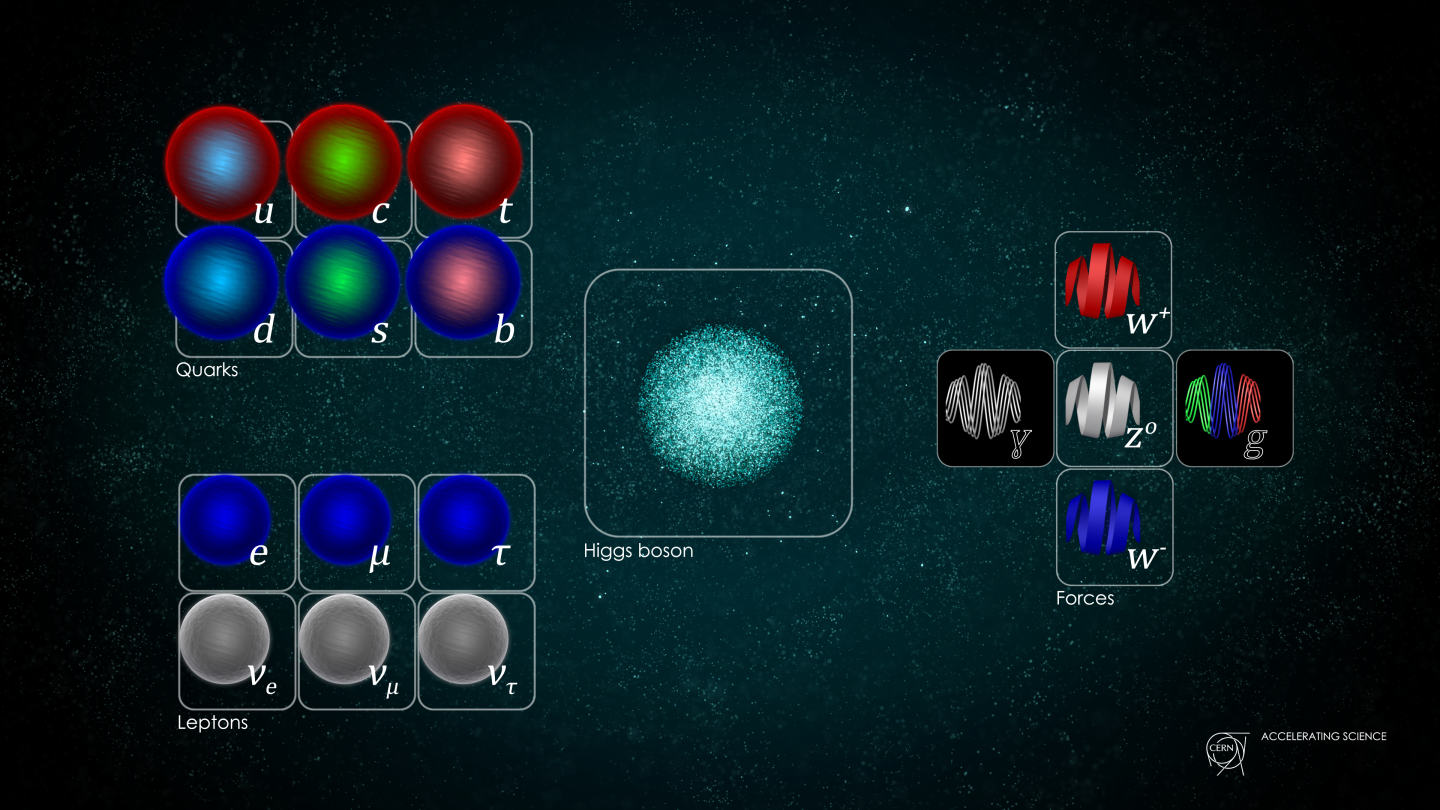
\includegraphics[width=\linewidth]{sm}
	\caption{Standard Model of Particle Physics, taken from \cite{sm}}
	\label{fig:sm}
\end{figure}

To follow is running coupling constant and missing resonances
\section{Photoproduction of Pseudoscalar Mesons}
$$\int_0^\infty\frac{\sin \alpha\beta x}{\gamma x}$$
\section{Polarization Obervables and the Complete Experiment}
bla
\section{Motivation and Structure of this Thesis}
bla